\chapter{Evaluation}
This chapter lists the pros and cons of available Technologies.
On this basis was evaluated, which hardware is suitable.

\section{Wakeup Receiver}
In this semester thesis, two different implementations of the wakeup receiver technology were compared.
The AS3933 from AMS and the RFicient from the \acf{fraun} which kindly provided an evaluation kit before the actual release of the product.
This section first introduces both products, before comparing them with a series of tests in a for this application realistic environment.

\subsection{AS3933}
The AS3933 is a low frequency wakeup receiver, which uses \acs{ask} to modulate a carrier frequency between 15-150\,kHz.
The transmitter sends a manchester encoded, programmable wakeup pattern of length 16 or 32 bit.
If this pattern is detected on the receiver end, a wakeup interrupt is generated.
It is also possible to disable the the pattern decoder to run the chip in a frequency detection mode, where a wakeup interrupt is generated as soon as any pattern on the specified frequency is received.
More important features on the receiver end are:
\begin{itemize}
	\item[-] Receiver sensitivity $80\,\mu\text{V$_{\text{RMS}}$}$
	\item[-] Current consumption in 3-channel listening mode $2.3\,\mu\text{A}$
	\item[-] Operating supply range $2.4\,\text{V}-3.6\,\text{V}$
	\item[-] Three antennas (enables 3D detection)
	\item[-] Channels  individually selective to reduce power consumption
\end{itemize}
The low power consumption makes it possible run the receiver in listening mode below $8.3\,\mu\text{W}$\cite{as3933}.

The demo kit comes with a \acs{gui}, which enables the user to set the parameters as desired.

\subsection{RFicient}
The Rficient from the \acs{fraun} uses \acs{ook} to modulate a 868\,MHz signal.
It can either run in pure wakeup mode, where the receiver generates an interrupt as soon as a code is received or a selective mode, where a 16 bit wakeup preamble needs to match the receiver. 
After the preamble is detected, the data rate can be changed to transfer more bits which can be sent over an \acs{spi}-bus to a connected device.
This way, it is possible to transmit data bits after the actual wakeup.
Data rates can be set in a range between $256\,\text{bp/s}-32\,\text{kbp/s}$.
The most important features are:
\begin{itemize}
	\item[-] Receiver sensitivity -80\,dBm
	\item[-] Energy consumption $3\,\mu\text{A}$ at $1.5\,\text{V}$ (data rate 1 kbit/s)
	\item[-] Unidirectional data transfer possible	
\end{itemize}
The power consumption therefore is in listening mode (data rate = 1 kb/s) $4.5\,\mu\text{W}$.

Just as the AS3933, the RFicient demo kit comes with a \acs{gui}, which enables the user to set the important parameters and even access the register directly \cite{rficient}.

\subsection{Test run in realistic environments}
It is not easy to compare the two wakeup receivers directly, since one operates in the 

\begin{figure}[ht]
	\centering
	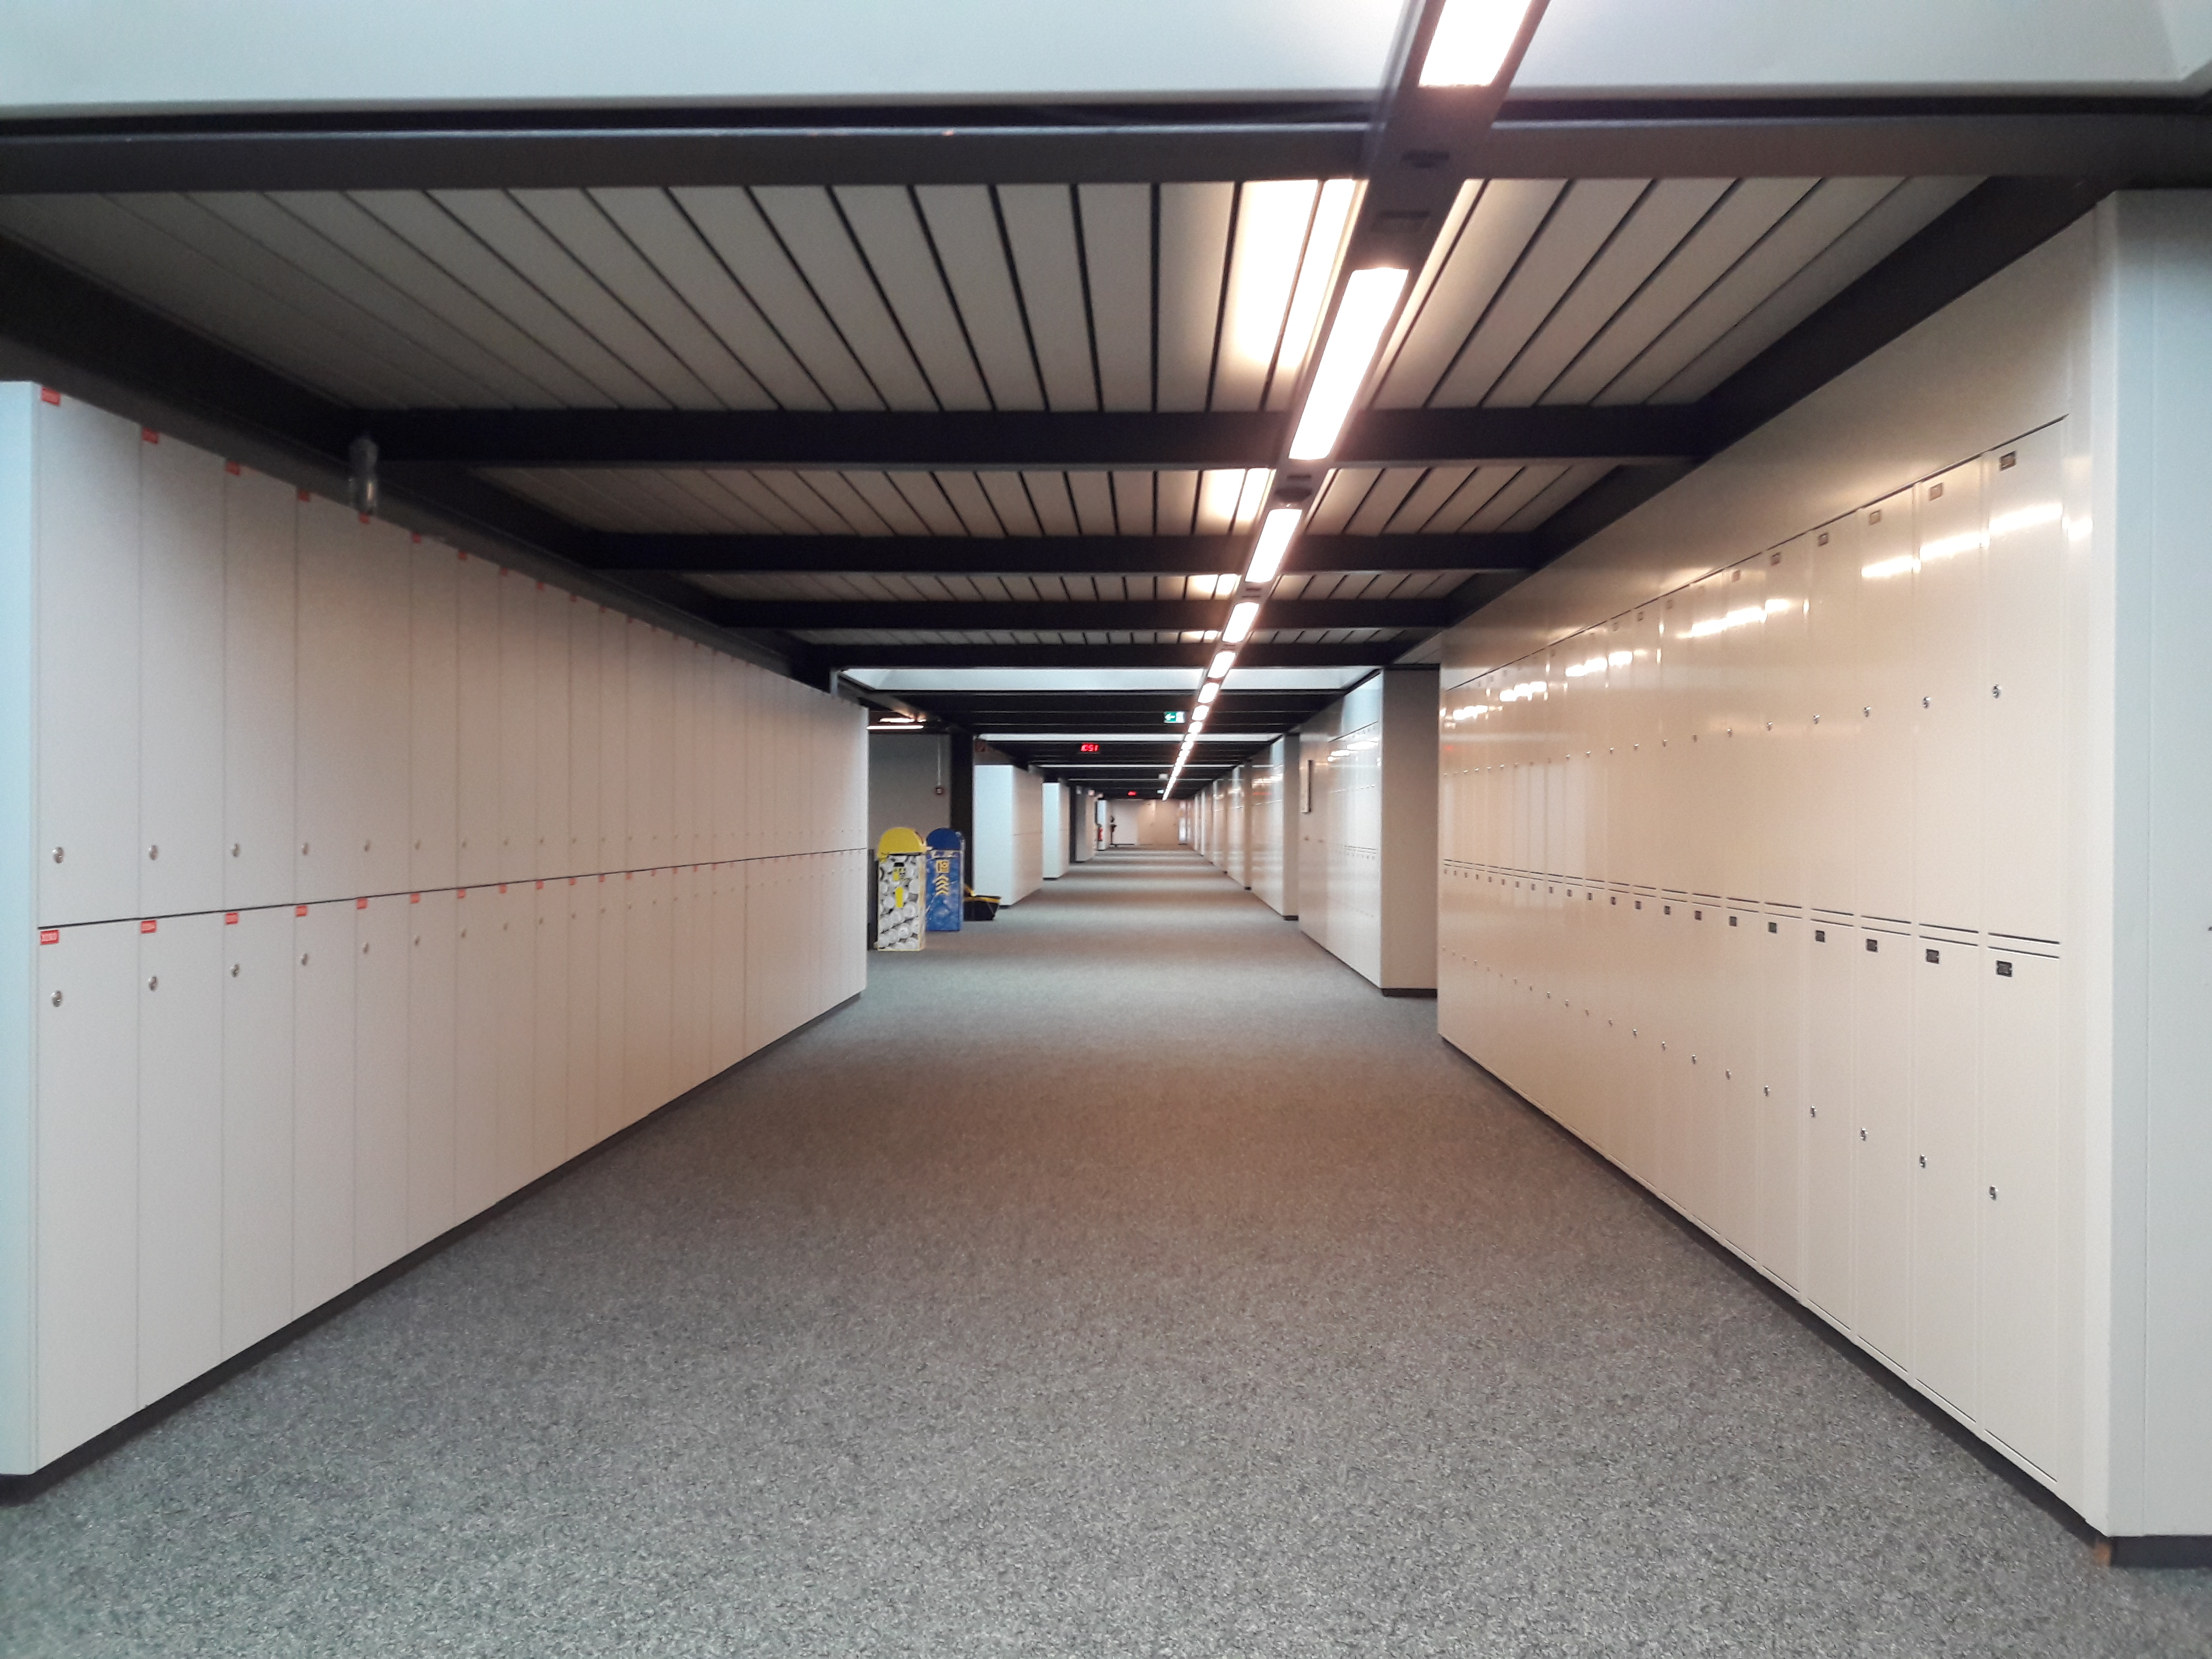
\includegraphics[width=0.9\textwidth]{3-evaluation/graphics/env1.jpg}
	\caption{Test environment 1 (filler)\label{evaluation:env1}}
\end{figure}

\begin{figure}[ht]
	\centering
	
\includegraphics[width=0.9\textwidth]{3-evaluation/graphics/env2.jpg}
	\caption{Test environment 2 (filler)\label{evaluation:env2}}
\end{figure}